\chapter{CTMC}

\section{Basics, Center of Mass and laboratory systems}

In the laboratory system the equations for each of the $n$ particles is
\begin{eqnarray*}
  \dot{\bm{r}} &=& \bm{p}/m \\
  \dot{\bm{p}} &=& - \nabla_{r} V(r) = \bm{F}(r)
\end{eqnarray*}
where $F(r)$ is the total force exerted over the particle.


In the center of mass frame the movement equations for the Jacobi
coordinates are given by
%
\begin{eqnarray} \label{Q:CTMC2}
  \dot{\bm{r}}_{j} & = &  \frac{\bm{k}_{j}}{m_{j}} \nonumber \\
  \dot{\bm{R}}_{j} & = & \frac{\bm{K}_{j}}{\mu_{j}}
  \nonumber \\
  \dot{\bm{k}}_{j} & = & \sum_{\ell = P,T,N} \nabla_{\bm{r}_{\ell}} V_{\ell} \;
  \left( \frac{\partial \bm{r}_{\ell}}{\partial \bm{r}_{j}} \right)_{\bm{R}_{j}}
  = \sum_{\ell = P,T,N} \bcal{M}^{11}_{\ell j} \;\, \nabla_{\bm{r}_{\ell}}
  V_{\ell}(\bm{r}_{\ell}) \nonumber \\
  \dot{\bm{K}}_{j} & = & \sum_{\ell = P,T,N} \nabla_{\bm{r}_{\ell}} V_{\ell} \;
  \left( \frac{\partial \bm{r}_{\ell}}{\partial \bm{R}_{j}} \right)_{\bm{r}_{j}}
  = \sum_{\ell = P,T,N} \bcal{M}^{12}_{\ell j} \;\, \nabla_{\bm{r}_{\ell}}
  V_{\ell}(\bm{r}_{\ell}) \; ,
\end{eqnarray}

\section{Sturmian-like Wigner distributions}
\label{S:sturmian-like-wigner}

In the CTMC method with microcanonical distributions the classical spatial
density is too compact compared to the quantum one and vanishes identically
beyond $r = 2$ a. u.  In the standard CTMC method (as we ussually use it) the initial
state of the H(1s) atom is described by means of a modified Wigner distribution
\parencite[see for instance][]{Hardie1983JPBp1983,Wood1997PRAp3701}. This method utilizes a discrete
superposition of microcanonical ensembles in order to provide a good
approximation to the H(1s) initial radial distribution. This description of the
initial state slightly degrades the momentum distribution.

 A possible similar approach that does not change neither the momentum
distribution nor the binding energy has been suggested (to me) by S.~Otranto. First, we observe
that the momentum distribution of hydrogen atoms
\begin{equation}\label{Q:class-momen-distr-hydro}
  \tilde{\rho}_{n}(\bm{p}) = \sum_{\ell, m} \left| \varphi_{n,\ell,m}(\bm{p})\right|^{2} 
  = \frac{8 }{\pi^{2}} \, \frac{p_{E}^{5}}{\left( p^{2} + p_{E}^{2} \right)^{4}}
\end{equation}
with the binding energy $\varepsilon=p_{E}^{2}/2 m_{T}$, is independent of the
nucleus charge $Z_{T}$. This is particularly important because it will allow us
to expand the radial momentum distribution in microcanonical distributions for
hydrogenlike atoms where each term has the same fixed binding energy and
momentum distribution. This is similar to an expansion of wavefunctions in
Sturmian states in quantum-mechanics.

The main disadvantage of this method is that the dynamics of the system does not
correspond to the hydrogen atom but to a hydrogen-like atom with a different
charge.

\subsection{Description of the method}
\label{S:description-method}

The quantum-mechanical spatial distribution is given by $\rho_{QM}(\bm{r})$
while its classical counterpart for a hydrogenic atom of charge $Z_{T}$ is given by
\begin{equation}\label{Q:class-spati-distr-hydro}
  \rho_{Cl}(Z_{T}, \varepsilon, \bm{r})
\end{equation}

We will approximate the quantum-mechanical density as
\begin{equation}\label{Q:fitti-densi}
  \rho_{QM}(\bm{r}) \approx \sum_{j=1}^{n} \omega(j) \, \rho_{Cl}(Z_{T}(j), \varepsilon, \bm{r}) \quad, \qquad
  \sum_{j=1}^{n} \omega(j) = 1.
\end{equation}

The simplest approach would be to fix $n$ and $n$ values for $Z_{T}$ in order to
obtain $\omega(j)$ by a least-square fitting. A better approximation would be to
derive from the minimization also the values of $Z_{T}(j)$.

\section{Acceleration of convergence for large times}
After one of the relative energies $\varepsilon_{j}$ has converged. We
can decouple the movement of the pair of particles with relative
$\bm{r}_{j}$ from the movement of the third respect to their center of
mass. Let's suppose that this two-fragment state has been reached. The
position and momenta of Jacobi are ($\bm{r}_{0},\bm{R}_{0}$) and
($\bm{k}_{0},\bm{K}_{0}$). These can refer to $T,P$ or $N$.

Fisrt of all, we note that the magnitude of the impulse will be given by energy conservation. For infinite time, the magnitude of the relative momentum is given by
\begin{equation}
  \label{Q:ctmc_magnitude}
p_{\infty}^{2}= 2 m_{0} E = 2 m_{0} \left(V(\bm{r}_{0} + \frac{\bm{k}^{2}_{0}}{2 m_{0}})  \right)
\end{equation}

We want to solve the problem of scattering with initial condition set
to a finite distance, as shown in figure \ref{f:cond-in}

%\begin{floatingfigure}[r]{7cm}
\begin{figure}[h]\label{f:cond-in}
\centering
%  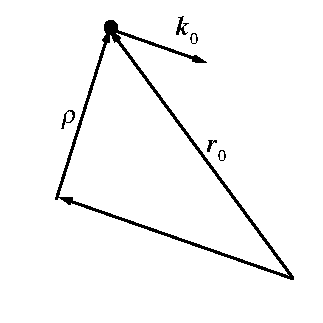
\includegraphics[clip,bb=17 15 170 170,width=5cm]{cond_in}
\caption{Initial condition after one of the relative energies has
converged}
\end{figure}
%\end{floatingfigure}


The impact parameter $\brho$ is given by the component of the distance,
perpendicular to the initial relative momentum $\bm{k}_{0}$,
\begin{equation}\label{Q:rho}
\brho = \hat{k}_{\,0} {\times} \left( \bm{r}_{0} {\times} \hat{k}_{\,0} \right)
\end{equation}

The final momentum will be given by
\begin{equation}\label{Q:finalmom}
\bm{p} = p_{E} \, \cos{\theta} \, \hat{k}_{0}+ p_{E}\, \sin{\theta}\,
\hat{\rho}
\end{equation}
%
where $\theta $ is the angle between $\bm{k}_{0}$ and $\bm{p}$. Then,
we only need to solve the ``\textit{off-shell}'' scattering problem
\cite{Fiol2000JPBp2847}.

%\begin{floatingfigure}[r]{8.2cm}
\begin{figure}[!htpb]
  \centering
%  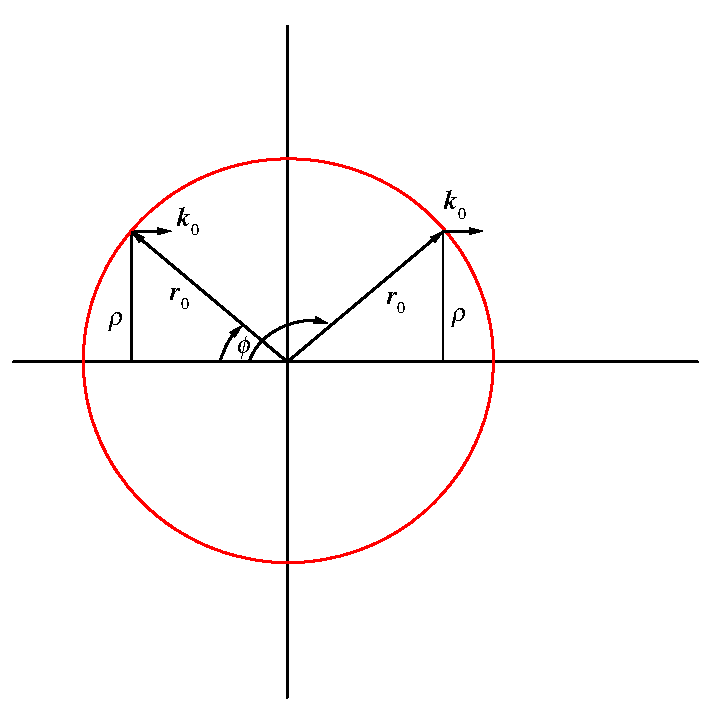
\includegraphics[width=7cm,bb=35 35 380 380,clip]{ctmc1}
  \caption{Problem equivalent to be solved.
  \label{f:ctmc1}}
\end{figure}
%\end{floatingfigure}


The solution of this problem is already known for Coulomb potential
$V(r) = Z/r$. In momentum space the trajectories of the particles are
circles of ratio $p_{R}$ and centered at $\bm{p}_{c}$ given by
\begin{eqnarray}\label{Q:circle-mom}
p_{R} &=& \frac{k_{0}}{2 \gamma} \, \frac{1}{\sin{\phi}} \nonumber \\
\\
\bm{p}_{c} &=& - \frac{k_{0}}{2 \gamma } \, \cot{\phi}\, \hat{\rho} +
\left( 1 + \frac{1}{2 \gamma} \right) \, \bm{k}_{0} \nonumber
\end{eqnarray}
where $\phi$ is the angle of the initial position ($\sin(\phi) =
\rho/r_{0}$) and $\displaystyle{\gamma = \frac{\left( k_{0}^{2}/2 m_{j}
\right)}{V(\bm{r}_{0})}}$.

%\begin{floatingfigure}[r]{8.2cm}
\begin{figure}%[!hptb]
  \centering
%  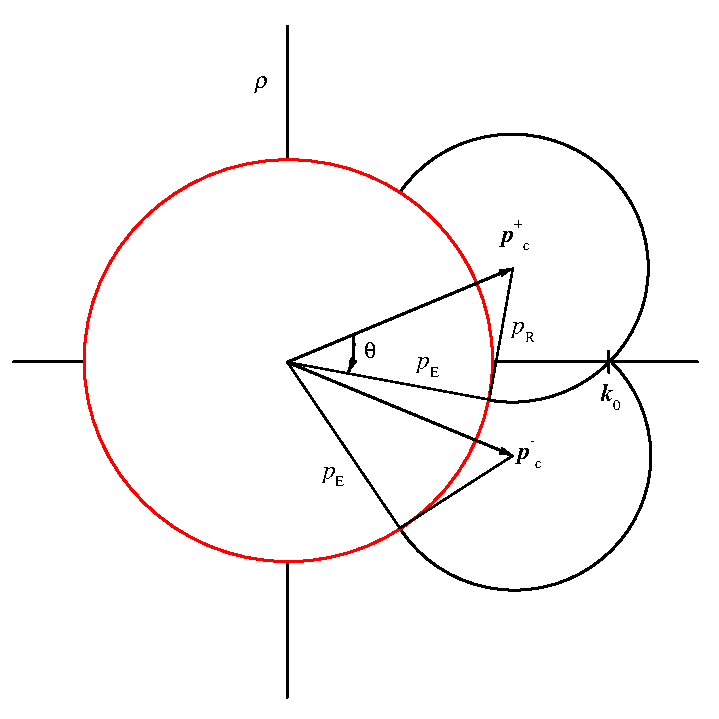
\includegraphics[width=7cm,clip,bb =35 35 380 380]{ctmc2}
  \caption{Solution of the problem in momentum space and definition of
  variables.
  \label{f:ctmc2}}
\end{figure}
%\end{floatingfigure}

While such a circle intersects the sphere of constant energy $p_{E}$ in
a rect angle (90$^{\circ}$), the angle of the final momentum relative to the
center $\bm{p}_{c}$ is given by

\begin{equation}\label{Q:angle}
\theta - \theta_{c} = {\rm sg}(Z) \, \arctan{\left( \frac{p_{R}}{p_{E}}
\right)} \ .
\end{equation}

The final momentum can be obtained replacing \ref{Q:angle} in
\ref{Q:finalmom}, with
\[
\theta_{c} = \arctan\left[(2 \gamma + 1) \, \rho / r_{0\, \|} \right]
\,.
\]

\section{Multiple-electron targets}

\subsection{Initialization of the target}
\label{S:Initi-targe}

First we set the electrons' momenta and coordinates fixing their
nucleus to the origin. This fixes their values to

\[
\bm{p}'_{j} = m_{j} \bm{p}_{T,j}/m_{T,j} \qquad \bm{r}'_{j} =
\bm{r}_{T,j}
\]

where $\bm{p}_{T}, \bm{r}_{T}$ are obtained in the center of mass
nucleus-electron (for both projectile target). The internal center of
mass velocity and position are
%
\[
M_{tot} \bm{v}_{cm} \equiv \sum_{j} \bm{p}'_{j}  \qquad M_{tot}
\bm{r}_{cm} \equiv \sum_{j} m_{j} \bm{r}'_{j}
\]

These two vectors have to be zero in the reference system attached to
the initial velocity of the whole fragment. At the same time the
relative velocities and distances between each electron and their
parent nucleus have to remain unchanged. Then constant velocities and
distances vectors must be subtracted to all momenta and positions such
that the new vectors verify simultaneously the following conditions
\begin{eqnarray*}
  0 &=& M_{N} \bm{r}_{N} + \sum_{j} m_{j} \bm{r}_{j} \\
  0 &=& M_{N} \bm{p}_{N} + \sum_{j} \bm{p}_{j} \\
\frac{\bm{p}_{j}}{m_{j}} - \frac{\bm{p}_{N}}{m_{N}} &=&
\frac{\bm{p}_{T,j}}{m_{T,j}}\, \bm{r}_{j}-\bm{r}_{N} = \bm{r}_{T}
\end{eqnarray*}

Finally, we have to translate these values to the initial position and
velocity of the fragment.

\section{Inclusion of tunneling}
\label{S:Inclu-tunne}

First we sketch the method used by Cohen \autocite{Cohen2001PRAp043412}. He proposed
to use the tunneling probability obtained in the semiclassical (JWKB)
approximation. Let's consider an atom immersed in an external
electromagnetic field. In the two-body center of mass system it is
equivalent to a particle of reduced mass $m_{\alpha}$ and charge
$Z_{\alpha}$ in a potential center $V_{\alpha}$. The tunneling
probability it is given by \cite{Galindo1990_QMvII}

\begin{equation}\label{Q:proba-tunne-JWKB}
\mathcal{P}_{\mathrm{tun}} \equiv T_{\mathrm{WKB}} = \exp{\left\{ -
\frac{2 \sqrt{(2 m_{\alpha})}}{\hbar} \int_{r_{1}}^{r_{2}} \left[
\mathcal{V}(\bm{r}) - \mathcal{V}(\bm{r}_{1})\right]^{1/2} d \bm{r}
\right\}} \, ,
\end{equation}
%
where $\bm{r}_{1}, \bm{r}_{2}$ are the turning points of the effective
potential $\mathcal{V}$ such that $\bm{r}_{2}$ is connected to the
continuum and $V(\bm{r}_{1})=V(\bm{r}_{2})$. It also is assumed that
the tunneling is instantaneous. The (reduced) particle is transported
from $\bm{r}_{1}$ to $\bm{r}_{2}$ while its velocity remains unchanged.

The first impression is that the potential in equation
\ref{Q:proba-tunne-JWKB} is given by
%
\begin{equation}\label{Q:effec-poten-JWKB}
\mathcal{V}(\bm{r}) = V(\bm{r}) + \frac{1}{2 m_{\alpha}}
\frac{L^{2}}{r^{2}} + Z_{\alpha} \bm{F}(t_{0})  \cdot \bm{r} \, ,
\end{equation}
%
where $L=\hbar (l+1/2) = \bm{k}_{\alpha} \cdot \bm{r}_{\alpha}$.
However we should check this.

The probability of tunneling must be evaluated every time the particle
reaches the position $\bm{r}_{1}$ or equivalently its momentum
(velocity) in the direction of the field vanishes ($\bm{k} \cdot
\bm{F}(t) =0$). Also the direction of the external field must be such
that it lowers the interaction potential in the direction that connects
$\bm{r}_{1}$ and $\bm{r}_{2}$ ($Z_{\alpha} \bm{F}(t_{0})  \cdot \bm{r}
< 0$).

\subsection{Hydrogen atom in an immersed field}
\label{S:Hydro-atom-immer-field}

%%% Local Variables: 
%%% mode: latex
%%% TeX-master: "mainxs"
%%% End: 
